\begin{figure}[t!]
	\begin{tikzpicture}
		\begin{axis}[
		table/col sep=comma,
		xlabel={(a) {cifar10}.},
		ylabel={Validation loss},
		height=2.3in,
		width= 2.7in,
   		ticklabel style={font=\small, fill=white},
		xticklabel style={rotate=90, anchor=near xticklabel},
	    xtick={0,0.1,0.2,0.4,0.6,0.8,1},
    	xticklabels={dummy,0,50,100,150,200,250},
		]
		\end{axis}
		\node[inner sep=0pt] at (2.83,2.28) {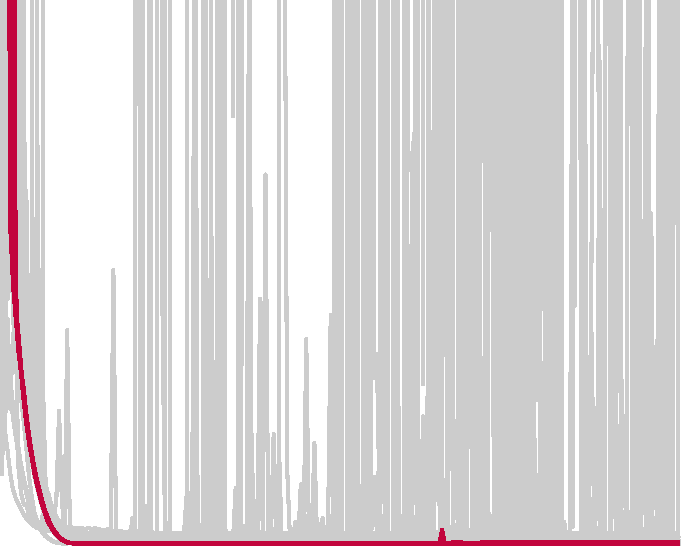
\includegraphics[width=0.4\textwidth]{figure4_a.pdf}};
	\end{tikzpicture}
	\begin{tikzpicture}
		\begin{axis}[
		table/col sep=comma,
		xlabel={(b) {cifar100}.},
		height=2.3in,
		width= 2.7in,
		ticklabel style={font=\small, fill=white},
		xticklabel style={rotate=90, anchor=near xticklabel},
		yticklabels={,,}
	    xtick={0,0.1,0.2,0.4,0.6,0.8,1},
    	xticklabels={dummy,0,50,100,150,200,250},
		]
		\end{axis}
		\node[inner sep=0pt] at (2.83,2.28) {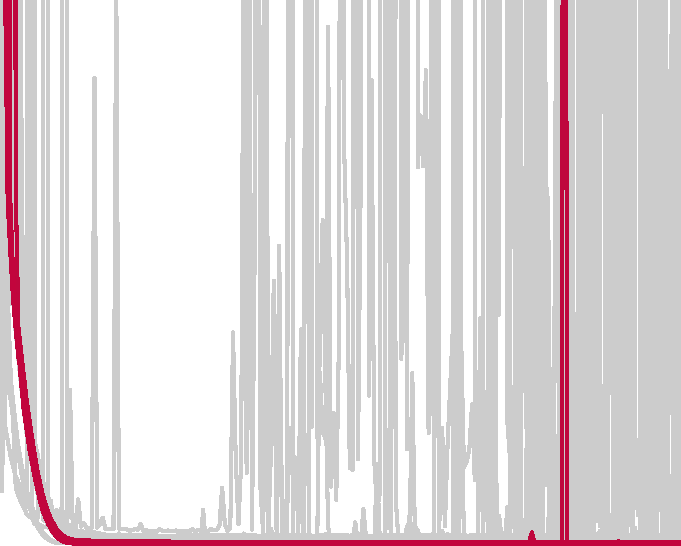
\includegraphics[width=0.4\textwidth]{figure4_b.pdf}};
	\end{tikzpicture}
\caption{The experiments show the mean squared error loss function on the validation dataset. We trained a total of $392$ neural nets $\approx 100$ times per dataset. Each line represents one neural net as an averaged loss function. The architecture can be found in Sect. \ref{subsec:invertibleneuralnets}, Appx. \ref{appx:invarch} and Fig. \ref{architecture}. The dimension of the net is chosen as a multiple of $2$, i.e. $2,4,6, \cdots, 784$. The {\color{brick} $\bullet$}--marked loss functions are parameterized above the determined threshold from Tab. \ref{stats}. The gray loss functions are below the defined threshold.}
\label{costfunctions}
\end{figure}